
\begin{figure}[!htbp]
    \begin{centering}
        \subfloat[Memory needed during iteration when correcting 25kb matrix]
        {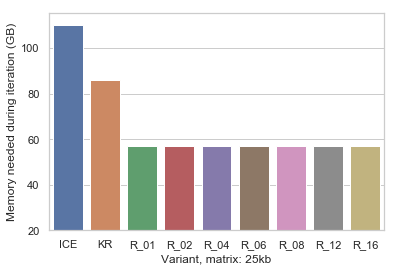
\includegraphics[scale=0.5]{figures/results/memiter_multi_25}}
        \subfloat[Maximum resident set size when correcting 25kb matrix]
        {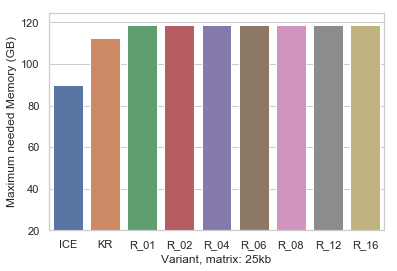
\includegraphics[scale=0.5]{figures/results/maxresident_multi_25}}
        \caption[Multicore Memory comparison]
        {\textbf{Multicore Memory needs} for correcting the 25kb matrix. Memory
        needs stay the same in all versions. Based on the numbers, there is no
        difference between the single-core version and any multi-core version
        regarding memeory usage.}
        \label{fig:memmulti}
    \end{centering}
\end{figure}

